\documentclass[italian,10pt,a4paper]{article}
\usepackage[T1]{fontenc}
\usepackage{babel}
\usepackage{geometry}
\usepackage{amsmath}
\usepackage{amsthm}
\usepackage{amssymb}
\usepackage{listings}
\usepackage{graphicx}
\usepackage{hyperref}
\usepackage[htt]{hyphenat}
\usepackage{cleveref}
\usepackage{xspace}
\usepackage{braket}
\usepackage{soul}
\usepackage{semantic}
\usepackage{mathtools}
\usepackage{subcaption}
\usepackage{framed}
\usepackage{cancel}
\usepackage{mdframed}
\usepackage[dvipsnames]{xcolor}
\newtheorem{theorem}{Teorema}
\newcommand{\bitem}[1]{\item\textbf{#1:}\xspace}
\newcommand{\aaa}[1]{\color{Purple}\text{#1}}
\lstset{
	basicstyle=\ttfamily\footnotesize,
	mathescape, 
	tabsize=4,
	breakatwhitespace,
	breaklines,
	breakautoindent,
	escapeinside={§}{§},
	numbers=left,
	numberstyle=\tiny,
	backgroundcolor=\color{gray!5},
	keywordstyle=\color{Blue},
	commentstyle=\color{Green},
	stringstyle=\color{Red},
	language=c		
}
\newcommand{\gcheck}{{\color{Green}\Large\checkmark}}
\title{Verifica automatica di programmi}
\author{Riccardo Torre}
\begin{document}
	\maketitle
%	\tableofcontents
	\section{BubbleSort}
\paragraph{Definizione di Partitioned}
$$\overbrace{\texttt{Partitioned($a,l_1,u_1,l_2,u_2$)}}^P \equiv \forall i\ \forall j \colon l_1 \le i \le u_1 < l_2 \le j \le u_2 \implies a[i]\le a[j]$$
\paragraph{Definizione di Sorted} $$\overbrace{\texttt{Sorted($a,l,u$)}}^S \equiv \forall i\ \forall j \colon l \le i \le j \le u \implies a[i]\le a[j]$$
\begin{lstlisting}
	§\aaa{pre: $\top$}§
	§\aaa{post: $\texttt{sorted}(rv,0,|rv| -1) $}§
	
	int[] BubbleSort(int[] a0){
		for §\aaa{@L1: $-1\le i < |a| \land \overbrace{P(a,0,i,i+1,|a| -1)}^A\land \overbrace{S(a,i,|a| -1)}^B$}§
		(int i := |a| -1; i > 0; i := i+1){
			for §\aaa{@L2: $1 < i < |a| \land 0 \le j \le i \land A \land B \land P(a,0,j-1,j,j)$}§
			(int j := 0; j < i; j := j+1)
				if(a[j] > a[j+1]){
				int t := a[j];
				a[j] := a[j+1];
				a[j+1] := t;
			}
		}
		return a;
	}
\end{lstlisting}

\subsection{Cammini elementari di BubbleSort}
\begin{figure}[tbph]
	\centering
	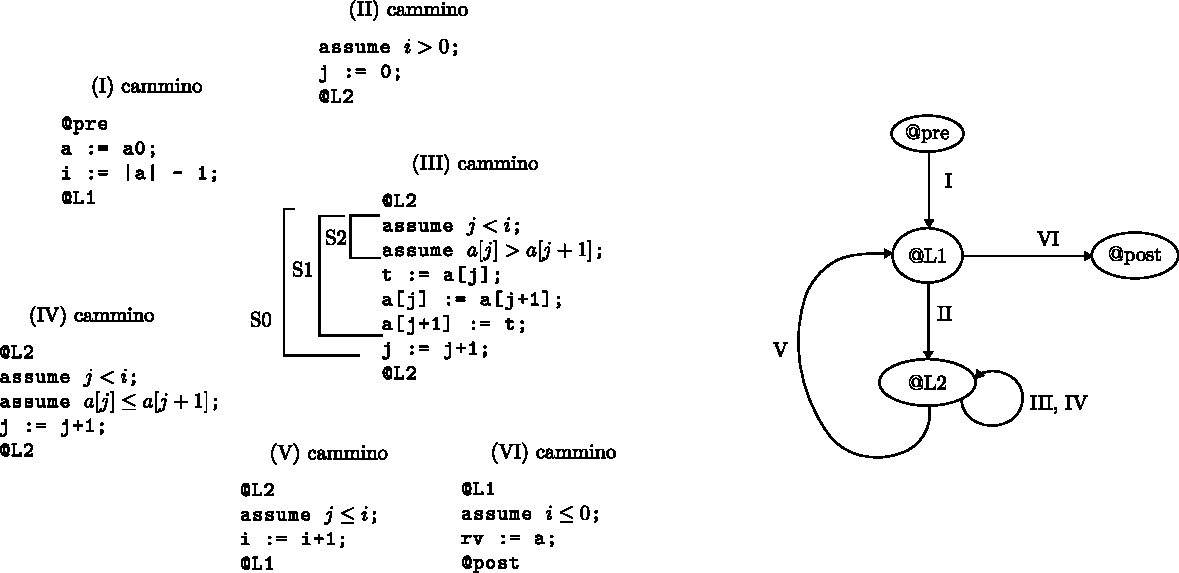
\includegraphics[width=\linewidth]{bubblesort}
	\caption{cammini minimi e grafo di BubbleSort}
	\label{fig:bubblesort}
\end{figure}
\paragraph{Inizio ciclo esterno}$P(a,\overbrace{0}^{l_1},\overbrace{|a| -1}^{u_1},\overbrace{|a|  \cancel{-1} \cancel{+1}}^{l_2}, \overbrace{|a| - 1}^{u_2} )$ è vera a vuoto perché $\not \exists j$ che verifica. Applichiamo la definizione di \texttt{Partitioned}. $$\overbrace{\texttt{Partitioned($a,l_1,u_1,l_2,u_2$)}}^P \equiv \forall i\ \forall j \colon l_1 \le i \le u_1 < l_2 \le j \le u_2 \implies a[i]\le a[j]$$ Sostituendo si ottiene $P(a_0,0,|a_0| -1, |a_0|, |a_0| -1) \equiv \forall i \forall j \colon 0 \le i \le |a_0| -1 < |a_0| \le j \le |a_0| -1 \implies a[i] \le a[j] $. Ma $\not \exists j \colon |a_0| \le j \le |a_0| -1$ perché $|a_0| -1 \not \le |a_0|$.
\paragraph{Inizio ciclo interno} $P(a,0,-1,0,0)$ è vera a vuoto poiché tra $0$ e $-1$ non esiste nulla ($\not \exists i \in [0,-1]$).
\subsection{Condizioni di verifica per i cammini del grafo}
\paragraph{Weakest precondition del cammino (I)} $wp(-1 \le i < |a|\land A \land B, \\\texttt{a := a0; i := |a| - 1;})\equiv (-1 \le |a| -1  < |a| \land  P(a,0,|a| -1,|a|,|a| -1)\land S(a,|a| -1,|a| -1), \texttt{a := a0})=(-1\le |a_0| - 1 < |a_0|\land  P(a_0,0,|a_0| -1, |a_0|, |a_0| -1)\land  S(a_0, |a_0| -1, |a_0| -1))$. 
\paragraph{Condizione di verifica per il cammino (I)}$T\implies (-1\le |a_0| - 1 < |a_0|\land  P(a_0,0,|a_0| -1, |a_0|, |a_0| -1)\land  S(a_0, |a_0| -1, |a_0| -1))$ è vera perché:
\begin{itemize}
	\item $P$ è vera;
	\item $S$ è vera;
	\item $-1 \le |a_0| -1 < |a_0|$ vera anche per $|a_0| = 0$.
\end{itemize}
\paragraph{Weakest precondition del cammino (II)}$wp(1\le i < |a| \land 0 \le j \le i \land A \land B \land P(a,0,j-1,j,j), \texttt{assume i > 0; j := 0;})\equiv i > 0\implies  1 \le i < |a| \land 0 \le 0 \le i \land P(a,0,i,i+1,|a| -1)\land S(a,i,|a| -1) \land P(a,0,-1,0,0)$.
\paragraph{Condizione di verifica per il cammino (II)}$[-1 \le i  < |a| \land P(a,0,i,i+1,|a| - 1) \land S(a,i, |a| - 1)\land i > 0]\implies [ 1 \le i < |a| \land 0 \le i \land P(a,0,i,i+1,|a| -1)\land S(a,i,|a| -1)\land P(a,0,-1,0,0)]$. L'implicazione è vera.
\paragraph{Weakest precondition del cammino (III)}$wp(1 \le i < |a| \land 0 \le j \le i \land P(a,0,i,i+1,|a| -1)\land S(a,i,|a| -1)\land P(a,0,j-1,j,j),S_0)=wp(1\le i \le |a| \land 0 \le j+1 \le i \land P(a,0,i,i+1,|a| -1)\land S(a,i,|a| -1)\land P(a,0,j,j+1,j+1),S_1)=wp(1 \le i < |b| \land 0 \le j+1 \le i \land P(b,0,i,i+1,|b| -1)\land S(b,i,|b| -1)\land P(b,0,j,j+1,j+1),S_2)$
\begin{mdframed}
	\item \texttt{t := a[j]} diventa \texttt{t $\leftarrow$ }{\color{Green}\texttt{select(a, j)}}
	 \item \texttt{a[j] := a[j+1];} diventa \texttt{a $\leftarrow$ {\color{Red}store(a, j, select(a, j+1))}} \item  \texttt{a[j+1] := t;} diventa \texttt{a $\leftarrow$ {\color{Blue}store(a, j+1, t)}}
	 \item combinando la seconda e la terza formula si ottiene \texttt{a $\leftarrow$ {\color{Blue}store(\color{Red}store(a, j, select(a, j+1))\color{Blue}, j+1, t)}}e sostituendo \texttt{t} con la prima formula si ottiene \texttt{a $\leftarrow$ }\texttt{\color{Blue}store(\color{Red}store(a, j, select(a, j+1))\color{Blue}, j+1, \color{Green}select(a,j)\color{Blue})}$\equiv \texttt{b}$ dove \texttt{b} è una \textbf{variabile temporanea} di tipo array.
\end{mdframed}
dunque la weakest precondition per il cammino (III) risulta: $[j<i\land \texttt{select}(a,j)>\texttt{select}(a,j+1)]\implies [1\le i < |b| \land 0 \le j+1 \le i \land P(b,0,i,i+1, |b| -1)\land S(b,i,|b| -1)\land P(b,0,j,j+1,j+1)]$
\paragraph{Condizione di verifica per il cammino (III)}$[1 \le i < |a| \land 0 \le j \le i \land P(a,0,i,i+1,|a| -1)\land S(a,i,|a| -1)\land P(a,0,j-1,j,j)\land j < i \land \texttt{select}(a,j)>\texttt{select}(a,j+1)]\implies [1\le i < |b| \land 0 \le j+1 \le i \land P(b,0,i,i+1,|b| -1)\land S(b,i,|b| -1)\land P(b,0,j,j+1,j+1)]$.

L'implicazione è vera siccome \texttt{b} è il risultato di due \texttt{store} e allora $|b| = |a|$ ed è facile vedere che vengono le altre parti dell'implicazione.
\paragraph{Weakest precondition del cammino (IV)}$wp(1\le i < |a|\land 0 \le j \le i \land A \land B \land P(a,0,j-1,j,j, \texttt{assume j < i; assume a[j] $\le$ a[j+1]; j := j+1;}))\equiv[j < i\land select(a,j) \le select(a,j+1)]\implies[1 \le i  <|a| \land 0 \le j+1 \le i \land A \land B\land P(a,0,j,j+1,j+1)]$.
\paragraph{Condizione di verifica per il cammino (IV)}$[1 \le i < |a| \land 0 \le j \le i \land A \land B \land P(a,0,j-1,j,j)\land j < i \land select(a,j)\le select(a,j+1)]\implies [1 \le i < |a| \land 0 \le j+1 \le i \land A \land B \land P(a,0,j,j+1,j+1)]$. L'implicazione è vera.
	\section{BinarySearch}
\paragraph{Ricorsione}Correttezza parziale di funzioni ricorsive via generazione delle chiamate di funzione sui cammini elementari:
\begin{itemize}
	\item Asserzioni in chiamata;
	\item Sommario di chiamata:
	\begin{lstlisting}[caption={profilo della funzione f}]
		§\aaa{@pre: F[p1,...,pn]}§ // sono i parametri formali di una funzione f
		§\aaa{@post: G[P1, ... Pn, rv]}§ // con rv valore restituito
		typeo f(type p1, ... type pn)   
	  //typeo $\color{Green}\omega$ := f(e1, ... ,en); $\color{Green}\rightarrow$ chiamata di f
	\end{lstlisting}
	\item Occorre almeno un cammino che termini con \texttt{@R: F[e1,...,en]} applicando la sostituzione di \texttt{p1,...,pn} con \texttt{e1,...,en}.
	\item Dimostrare la validità della condizione di verifica associata a ogni cammino che termina. L'asserzione di chiamata serve a dimostrare che la chiamata della funzione soddisfa la precondizione delle funzione.
	\item Occorre almeno un cammino che includa il sommario di chiamata \texttt{assume G[e1,...,en, v]; $\omega$ := v;} dove $v$ è il valore restituito dalla funzione chiamata ed \texttt{e1,...,en} sostituiscono \texttt{p1,...,pn}.
\end{itemize}
Nell'analisi di funzioni ricorsive, i cammini elementari iniziano con la precondizione e finiscono con la postcondizione o con un'altra asserzione.
\subsection{Esempio}
\begin{lstlisting}
	§\aaa{@pre: x >= 0}§
	§\aaa{@post: rv >= x}§
	int g(int x){...}
\end{lstlisting}
Considerando una funzione che chiama $g$ $$\texttt{$\omega$ := g(n+1)}$$
$n$ è definita nella funzione che chiama $g$. Bisogna annotare la chiamata di $g$:
\begin{lstlisting}
	§\aaa{@R1: n + 1 $\ge$ 0}§ // $\color{Green}\rightarrow$ asserzione in chiamata
	$\omega$ := g(n+1);
\end{lstlisting}
\begin{enumerate}
	\item Almeno un cammino che termina su $@R$
	\item Almeno un cammino che includa: \texttt{... assume v $\ge$ n+1; $\omega$ := v;} con \texttt{v} valore gestito da $g$.
\end{enumerate}
\end{document}
